\chapter{Introduction}
\label{ch:intro}

\section{Motivation for Formalizing and Assembling Knowledge}
\label{ka_motivation}

The final step of knowledge discovery requires scientists to interpret and evaluate the patterns produced by data mining of pre-processed and transformed data \cite{Fayyad1996}. Classically, this step is guided by the knowledge of the scientist performing the interpretation. However, the quantity of knowledge the biomedical domain is increasing at an unprecedented rate with no signs of deceleration \cite{Bellazzi2014}. Even with the assistance of information retrieval technologies, it is overwhelming, if not impossible, for individuals or groups of researchers to be knowledgeable of the state-of-the-art in any but an incredibly specific topic.

The diversity of the content of the data in the biomedical domain is increasing as multi-modal and multi-scale experiments are more commonly used to investigate complex diseases. As experiments grow in complexity, so does the intellectual and temporal burden of interpretation and evaluation. A support system with the ability to reason over knowledge from both structured and unstructured sources in order to automatically interpret new data sets and generate hypotheses would provide a huge relief to this burden. The first step towards building a support system is to formalize knowledge into a computable form.

The most relevant is unstructured knowledge in biomedical literature. While previous efforts with manual curation have produced high-quality knowledge bases (e.g, \ac{UniProt} \cite{Bateman2017}, \ac{BRENDA} \cite{Placzek2017}, etc.), they also suffer from the burden of velocity and volume. Advances in automated and semi-automated information and relation extraction workflows are easing this burden. While the methods of information and relation extraction are not the focus of this thesis, a background on the schemata and formats used to store their result is necessary to proceed.

\section{Formats for Knowledge Assembly}
\label{ka_formats}

The most abstract level of knowledge, methodological knowledge, describes the formalisms through which knowledge can be represented. The two most common schemata for methodological knowledge are \ac{RDFS} and \ac{OWL}. They provide the faculty to describe the middle level, conceptual knowledge, which encodes the classes, relations, and constraints relevant to a given domain.  The most common conceptual knowledge formats in the biomedical domain are \ac{BioPAX}, \ac{SBML}, and \ac{BEL}. The most concrete level is factual knowledge, which consists of instances of these classes and relationships \cite{Marchetti2008}. These abstractions are illustrated in Figure 1.

\begin{figure}
\captionsetup{format=plain}
\makebox[\textwidth]{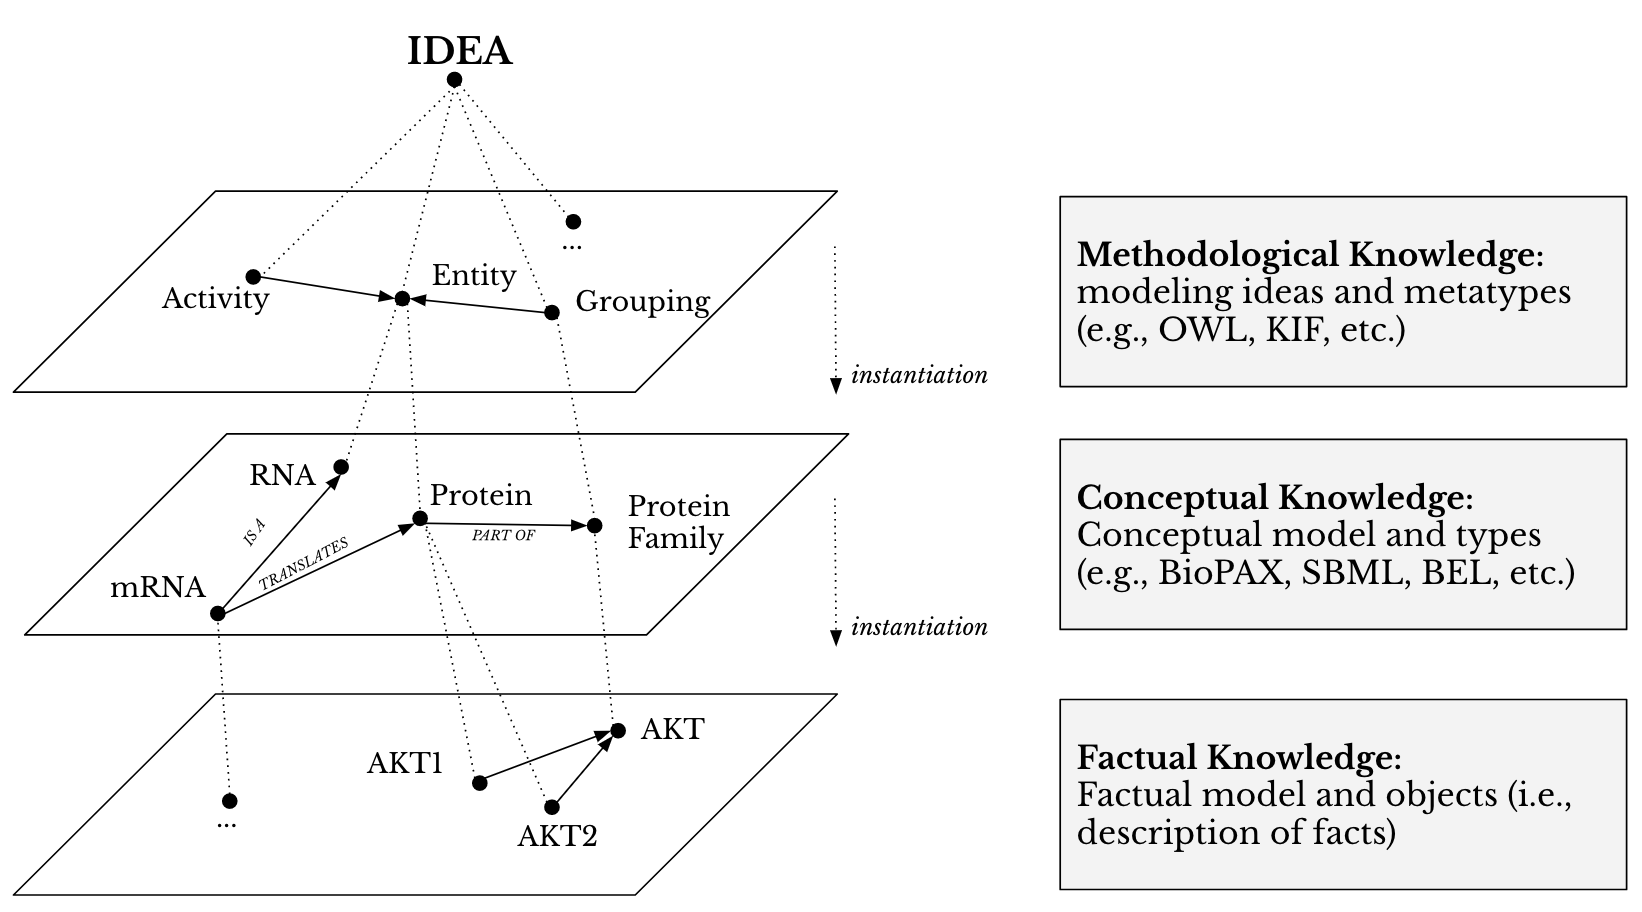
\includegraphics[width=160mm]{images/knowledge_types.png}}
\caption[Levels of Knowledge Abstraction]{The interplay of the three levels of knowledge abstraction in an example from the biological domain.}
\label{Fig:knowledge_types}
\end{figure}
	
\subsection{Resource Description Framework Schema}
    
\ac{RDF} uses triples of subjects, predicates, and objects to represent relations between concepts. Each resource in a triplet is backed by an \ac{IRI}. While its simple format grants it huge expressive power, RDF lacks structure or domain specificity. 

\ac{RDFS} is a set of concepts and predicates appropriate for describing knowledge at the conceptual level. Included are predicates for asserting class hierarchies (\verb|rdfs:subClassOf|), asserting memberships (\verb|rdf:type|), describing the domain and range of predicates (\verb|rdfs:domain|, \verb|rdfs:range|), and representing epistemological concepts such as classes, literals, and other data types \cite{Beckett2014}.

RDF and RDFS are supported by most popular programming languages with packages to serialize and deserialize \ac{RDF} in a variety of formats (e.g., \ac{XML}, N-Triples, turtle, etc.) and reason over \ac{RDFS}.
    
\subsection{Web Ontology Language}

Like \ac{RDFS}, \ac{OWL} consists of the methodological knowledge for modeling domain-specific knowledge. Its most simple form, \ac{OWL} Lite, enables the representation of classes, their properties, relations, and constraints. The most common form, \ac{OWL} \ac{DL}, contains the additional expressive power of descriptive logic over which inferences can be made. The most expressive form, \ac{OWL} Full, removes the remaining restrictions on \ac{OWL} \ac{DL} but paradoxically becomes undecidable and hinders automatic reasoning \cite{Marchetti2008}. The expressive levels of \ac{OWL} are depicted in Figure 2.

\begin{figure}
\captionsetup{format=plain}
\makebox[\textwidth]{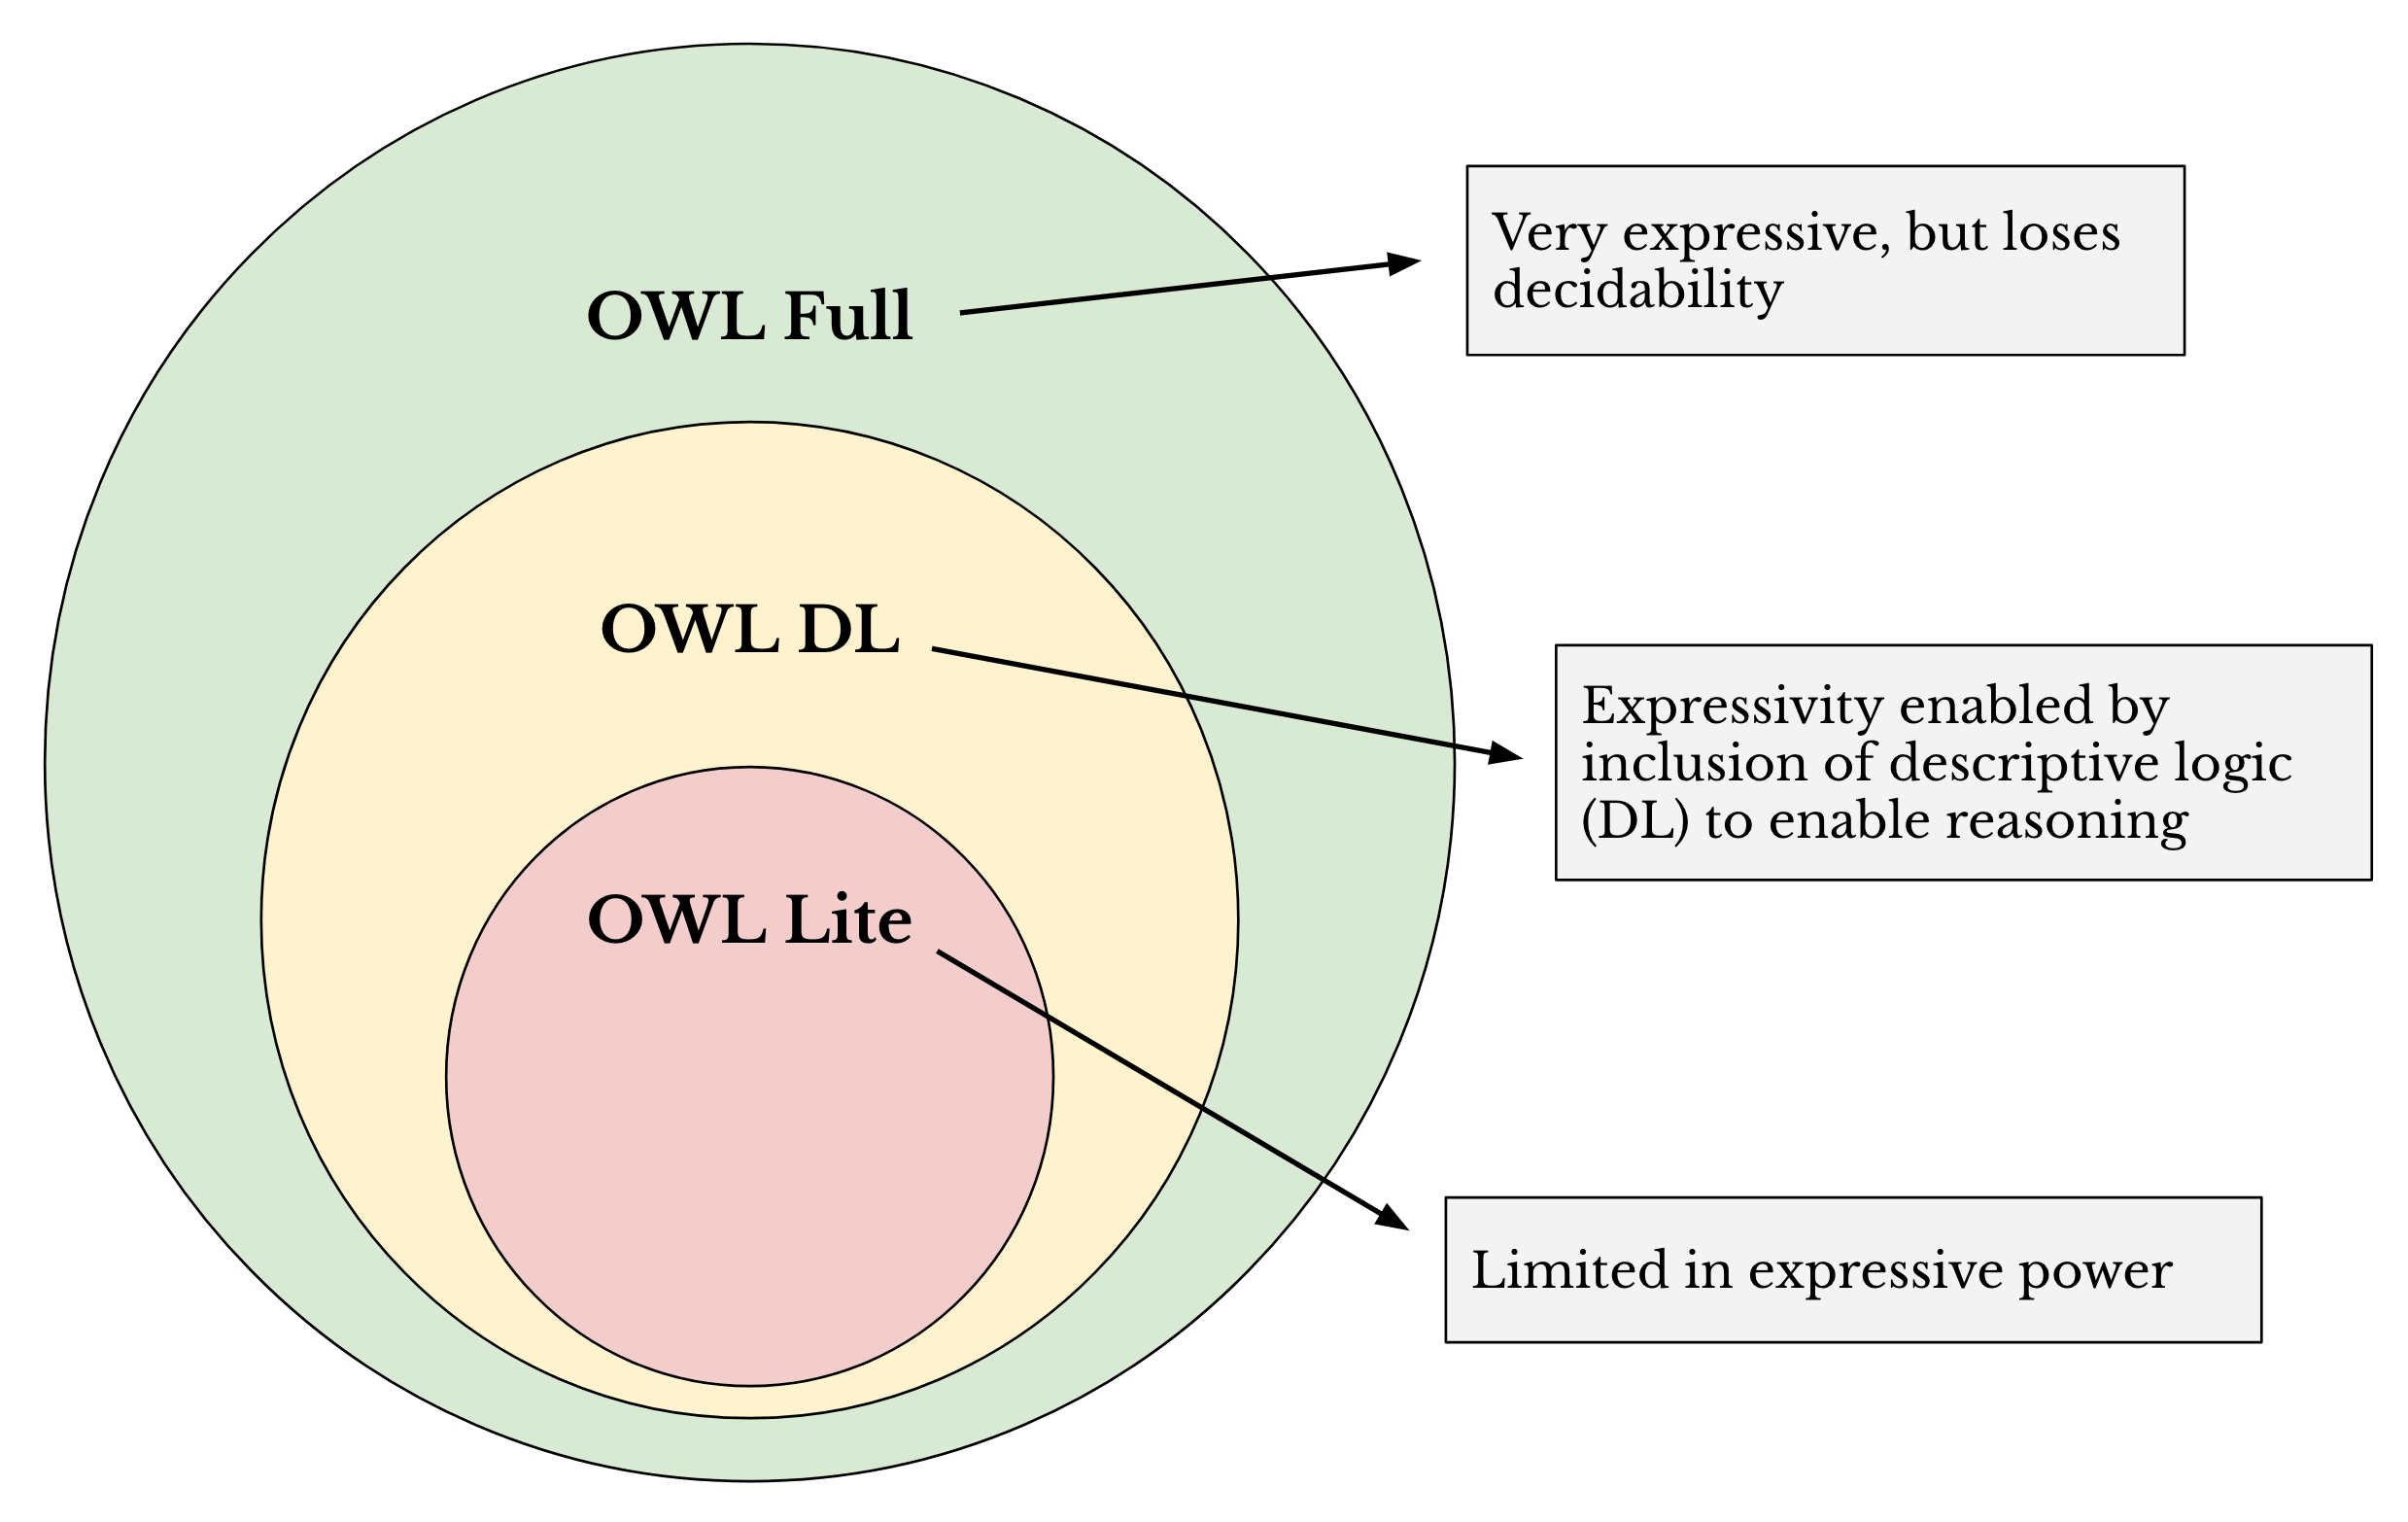
\includegraphics[width=160mm]{images/owl_types.png}}
\caption[Descriptive Levels of OWL]{The expressive levels of OWL ontologies. Adapted from \cite{Marchetti2008}.}
\label{Fig:owl_types}
\end{figure}

\ac{OWL} can be serialized to \ac{RDF}, RDF/XML, OWL/XML, Manchester, and several other formats. As an aside, the community of ontologists has historically used the Java programming language because of the definitive \verb|OWL API| \cite{owlapi} package. Because many bioinformatics tools have been written in the Perl, R, and Python scripting languages, they have been unable to easily make use of the most powerful reasoners available. Development on Python packages (e.g., \verb|OWLReady| \cite{owlready}, \verb|OntoSpy| \cite{ontospy}, \verb|obonet| \cite{obonet}, etc.) is beginning to enable Python programmers to make full use of the abstract concepts introduced in knowledge formalization.

\subsection{Biological Pathways Exchange Language}

\ac{BioPAX} uses \ac{OWL} to define the conceptual knowledge in the domain of biological pathways on the molecular and cellular level. Its ability to collect and index metabolic, signaling, molecular, gene-regulatory, and genetic interaction networks makes it an ideal exchange format for the growing number of pathway databases with varying specificities in regards to target organisms and disease indications \cite{Demir2010}.

This was realized with the aggregation of several pathway and interaction databases (e.g., BindingDB \cite{Gilson2016}, DrugBank \cite{Law2014}, IntAct \cite{Orchard2014}, \ac{KEGG} \cite{Kanehisa2017}, Reactome \cite{Fabregat2016}, WikiPathways \cite{Pico2008}, etc.) to form the Pathway Commons Database \cite{Cerami2011}. Immediately, this database enabled exploration of molecular interactions at the highest granularity. For example, it powers the Enrichment Map Cytoscape Plugin \cite{Merico2010} that was used to support data-driven analysis in identifying medulloblastoma subgraphs based on intratumoral heterogeneity \cite{Cavalli2017}.

\subsection{Systems Biology Markup Language}

\ac{SBML} uses a completely custom formalism defined with \ac{XMLS} to represent the dynamic and quantitative aspects of biochemical reactions, signal transduction, and gene regulatory networks \cite{Hucka2003}. Like \ac{BioPAX}, it provides the conceptual framework necessary to encode knowledge in the biomedical domain. \ac{SBML} also provides the basis for CellDesigner \cite{Funahashi2003}, which has been incredibly successful in allowing biologists without informatics backgrounds to diagram gene regulatory and biochemical networks as well as import them to graphical ordinary differential equation solvers and simulation workflows. 

\subsection{Biological Expression Language}

\ac{BEL} supports the assembly of context-specific qualitative causal and correlative relations between biological entities across multiple scales. Statements are assembled and serialized in \ac{BEL} Script with full provenance information including namespace references, relation provenance (citation and evidence), and relation metadata such as  biological context (i.e. anatomy, cell, disease, etc.) \cite{Slater2014}. The schemata of BEL relations and BEL Scripts are depicted in Figures 3 and 4, respectively.

Data-driven network analyses on \ac{BEL} knowledge assemblies have been successfully performed across a wide variety of clinical applications, including the identification of upstream controllers in hepatocytes \cite{Deehan2012}, mechanistic hypothesis generation for drug response \cite{Laifenfeld2014}, and patient stratification \cite{Laifenfeld2012} by using over-representation analysis techniques developed such as \ac{RCR} \cite{Catlett2013} and pathway topological analytical methods such as \ac{NPA} \cite{Martin2014}. 

\begin{figure}
\captionsetup{format=plain}
\makebox[\textwidth]{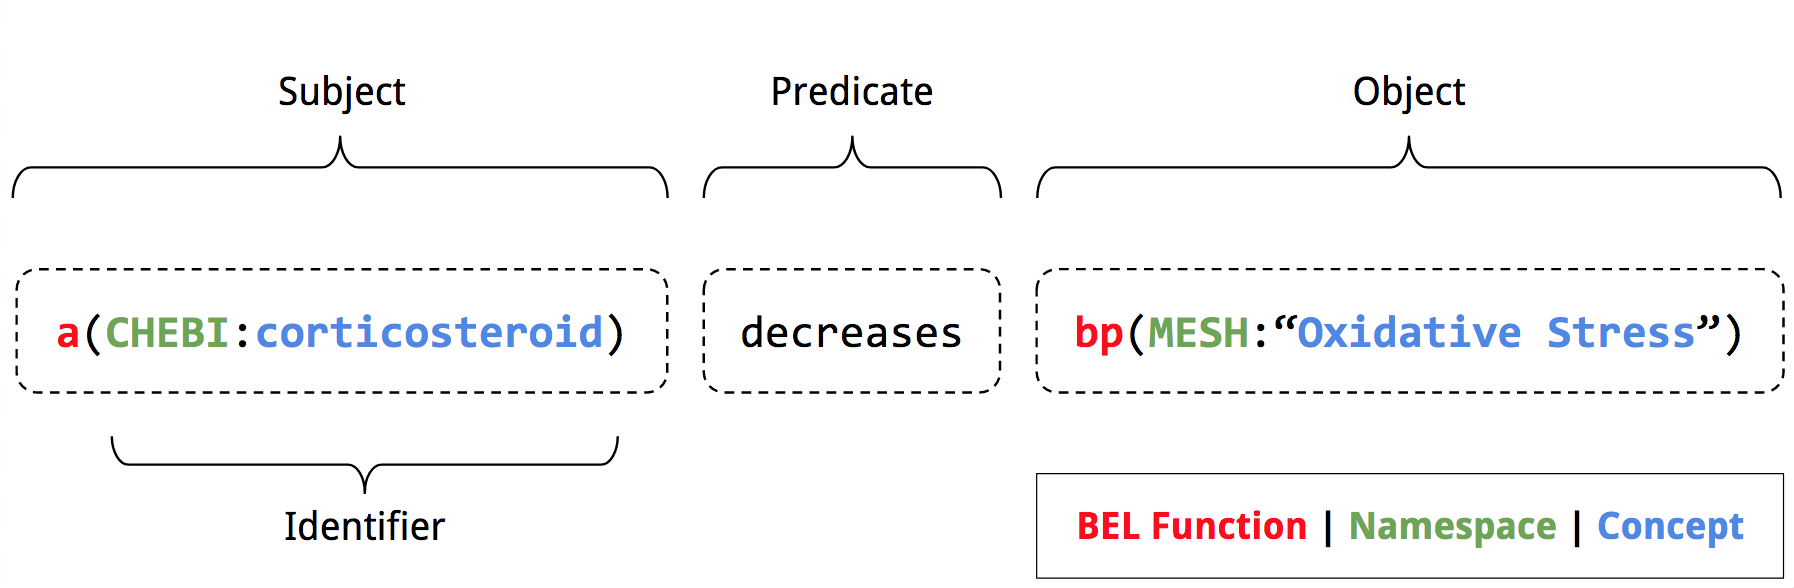
\includegraphics[width=160mm]{images/bel_relation.png}}
\caption[The Schema of a BEL Relation]{A BEL relation is encoded as a triplet containing a subject, a predicate, and an object. The predicate can represents the type of relation while the subject and object can either represent the abundance of molecular entities such as genes, proteins, chemicals, or more abstract concepts such as biochemical reactions, biological processes, and pathologies. Identifiers for these concepts use references to external namespaces (Figure 4B) to qualify their respective names. In this example, \ac{ChEBI} \cite{Hastings2013} is used to qualify chemicals and \ac{MeSH} \cite{ROGERS1963} for biological processes.}
\label{Fig:bel_relation}
\end{figure}

\begin{figure}
\captionsetup{format=plain}
\makebox[\textwidth]{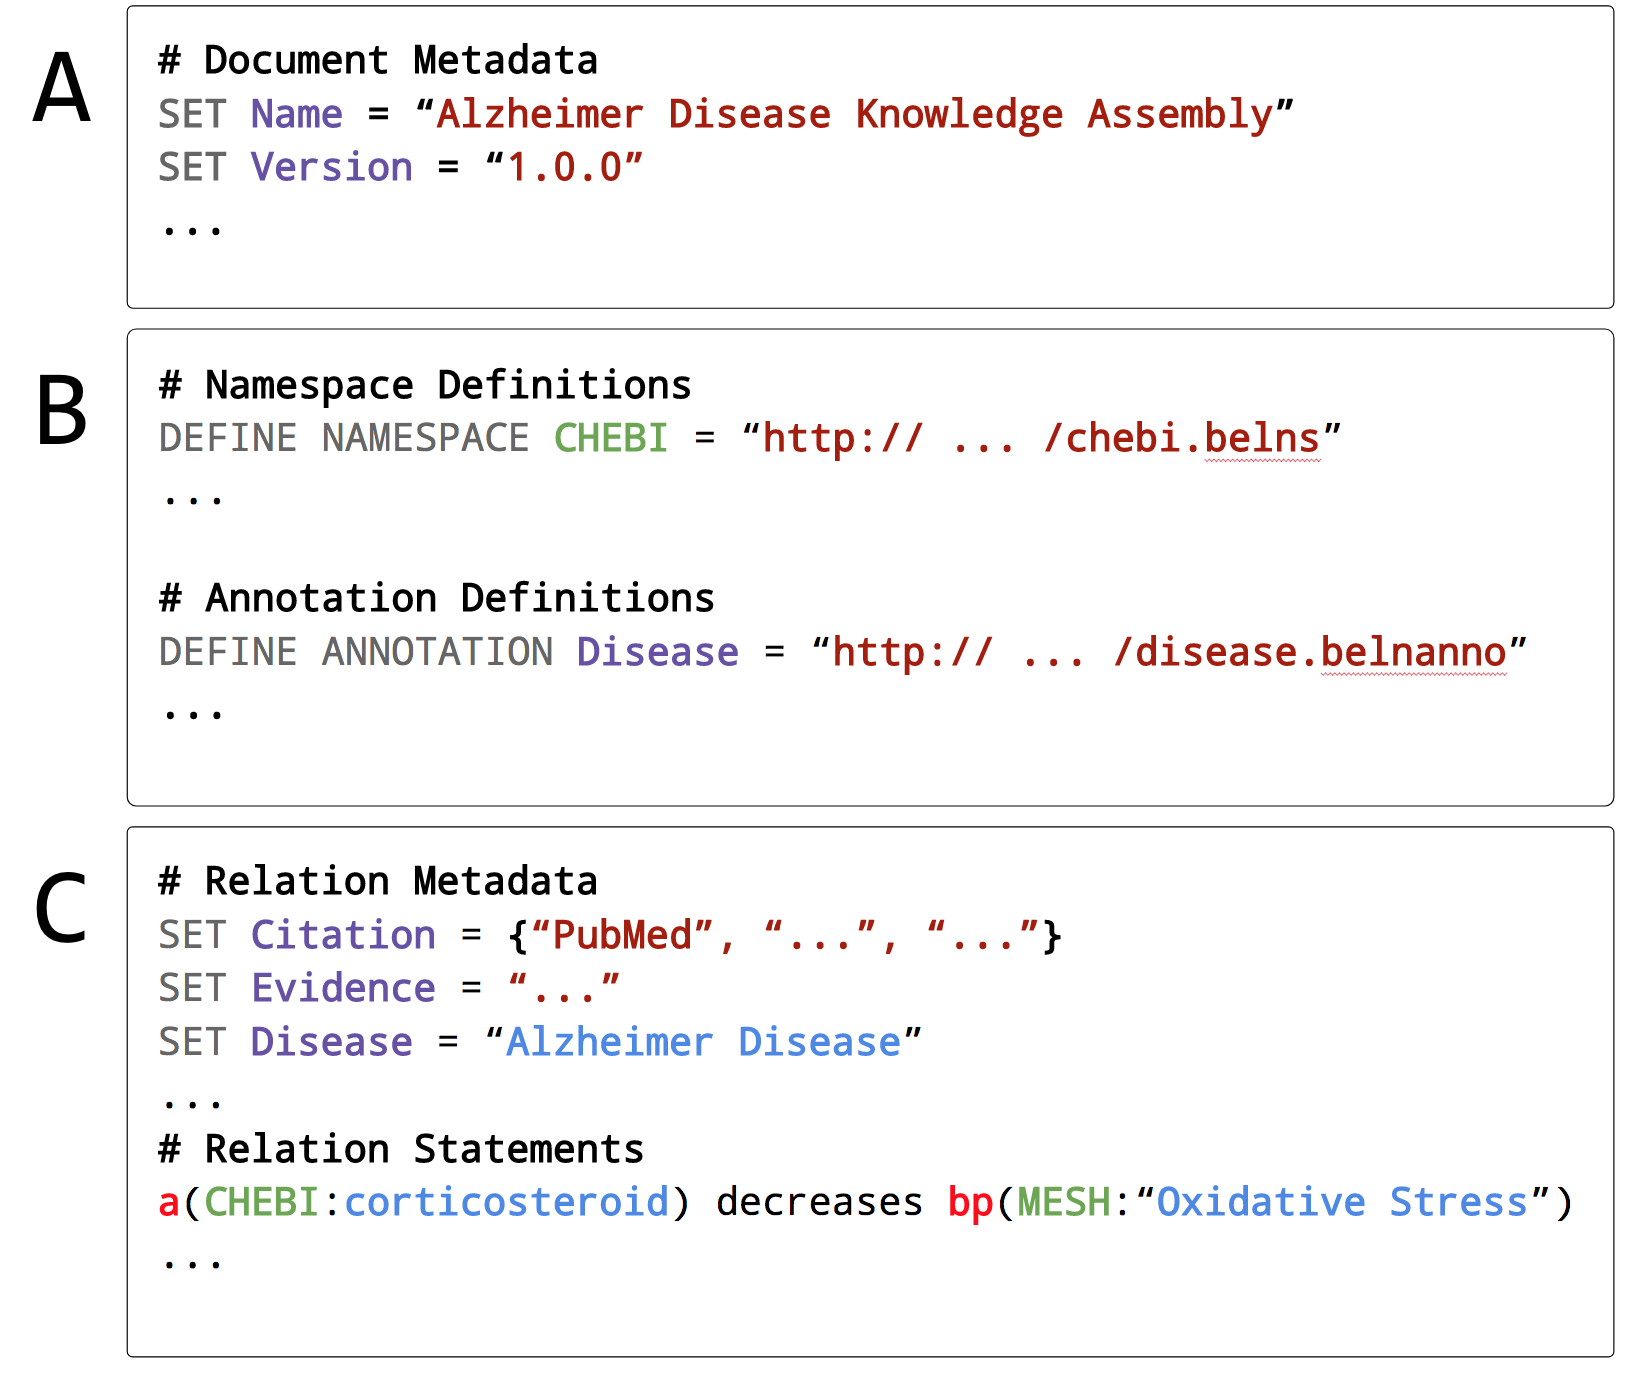
\includegraphics[scale=0.6]{images/bel_script.png}}
\caption[The Schema of a BEL Script]{A BEL Script contains three sections: A) the document metadata section provides provenance information such as the name, version, and author; B) the definitions section provides references to external resources that are used as identifiers and metadata in the relations section; and C) the relations section contains BEL relations and their metadata: minimally including a citation and evidence with the possibility to include additional information such as biological context (e.g. cell, anatomy, disease).}
\label{Fig:bel_script}
\end{figure}

BEL was developed by Selventa, a bioinformatics and computational biology consulting firm, to support knowledge-driven analysis of data. In 2012, they released the \ac{BEL} v1.0 specification as an open standard through the OpenBEL Consortium. However, the inability of BEL to express important concepts in molecular biology (such as genetic variants) prompted the \ac{BEL} v2.0 revision in 2014.

The foray into new disease areas and clinical indications has necessitated the assembly of knowledge on wider scales from the genetic to the phenotypic and population levels. While most modeling languages and data formats for assembling knowledge are insufficient for such a task, BEL possesses the faculty for capturing multi-scale knowledge. 

In the same way \ac{BioPAX} was successful at combining many molecular pathway and interaction database, \ac{BEL} has the potential to serve as a semantic integration platform through which knowledge and data across scales can be integrated and analyzed. \ac{BEL} can be used to reason over the previously untapped sources of chemogenomic and chemical genetic information in the realm of disease-disease, disease-protein, disease-chemical, and chemical-chemical networks.

Modeling interactions across scales is not without its issues. As biological processes, pathologies, and phenotypes represent collections of molecular interactions, they are prone to having excessive associative and correlative relations to other biological entities. This biases typical graph mining algorithms that rely on  graph traversals to visit these types of nodes, and therefore produce less meaningful results. While it is not within the scope of this thesis, there are many solutions for addressing these issues whose complexities vary from simple filtering to empirical traversal rules. or adding extra rules for traversals.

\section{Biological Applications}
\label{biological_applications}

\subsection{NeuroMMSig}

The work in this thesis was carried out in order to support the \ac{IMI} \cite{imisite} project, AETIONOMY \cite{aetionomy}. The goal of this project is to provide a taxonomy of neurodegenerative disease in order to support further development of clinical and computational methods to identify patient subgroups and classify individuals accordingly. 

The first step taken towards this goal was to encode the relevant knowledge surrounding \ac{AD}, \ac{PD}, and Epilepsy in BEL \cite{Kodamullil2015}. Next, a taxonomy of candidate mechanisms was curated in the \ac{NeuroMMSig} Knowledge Base and annotated to these knowledge assemblies \cite{Domingo-Fernandez2017}. These candidate mechanisms contain multiple causal pathways, correlative and associative relations, as well as other related information and are most appropriately named "subgraphs."
